\documentclass{standalone}

\usepackage{tikz}
\usepackage{amsmath}
\usepackage{unicode-math}

\usetikzlibrary{
  arrows, arrows.meta,
  calc,
}

\begin{document}
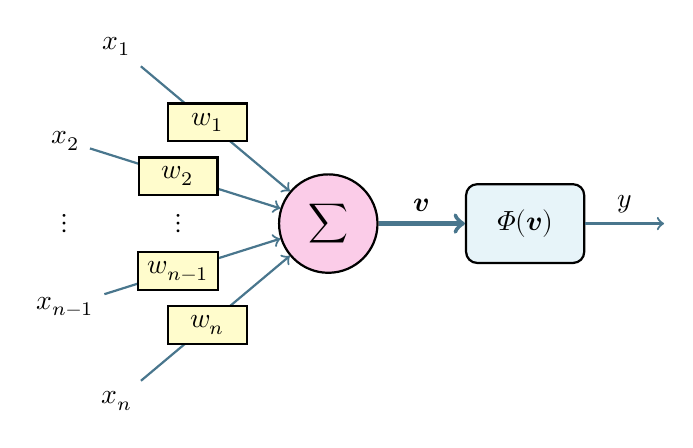
\begin{tikzpicture}[
  thick,
  arr/.style={cyan!50!black},
  larr/.style={arr, {Latex[round]}-},
  rarr/.style={arr, {-Latex[round]}},
  ]
  \node[draw=black, circle, minimum size=1.25cm, fill=magenta!20]
  (s) at (0,0) {$\displaystyle \sum$};
  \node[draw=black, rectangle, minimum height=1cm, minimum width=1.5cm, rounded corners, fill=cyan!80!black!10]
  (p) at (2.5,0) {$\varPhi(\mathbfit{v})$};

  \foreach \i/\a in {1/-40, 2/-17.5, n-1/17.5, n/40}{
      \node (x\i) at (180+\a:3.5) {$x_{\i}$};
      \draw[arr, -to] (x\i) -- (s);
      \node[rectangle, draw=black, fill=white, minimum width=1cm, fill=yellow!20]
      (w\i) at (180+\a:2) {$w_{\i}$};
    }
  \node at (-1.9, 0) {$\vdots$};
  \node at (-3.35, 0) {$\vdots$};

  \draw[ultra thick, arr, -to] (s) -- (p)
  node[midway, above, black] {$\mathbfit{v}$};
  \draw[arr, -to] (p.0) -- ++(1,0)
  node[midway, above, black] {$y$};
\end{tikzpicture}
\end{document}
